\clearpage
\section{Pianificazione}
La pianificazione, elaborata dal gruppo \emph{duckware}, è stata costruita sulla base delle scadenze temporali riportate al \hyperlink{scadenze}{punto 1.5} e con esse viene suddiviso lo sviluppo in cinque fasi raggruppate in due periodi:
\begin{itemize}
	\item \textbf{Investimento}
		\begin{itemize}
			\item Analisi;
			\item Consolidamento dei \markg{requisiti}.
		\end{itemize}
	\item \textbf{Preventivo}
	\begin{itemize}
		\item Progettazione architetturale;
		\item Progettazione di dettaglio e codifica;
		\item Validazione e collaudo.
	\end{itemize}
\end{itemize}
Ciascuna di queste fasi è stata scomposta in sotto-attività, che sono state svolte durante la fase stessa per facilitarne lo sviluppo. A ogni periodo è stata fissata una scadenza, ovvero il giorno di consegna dei materiali che sono stati prodotti dalle attività svolte. Tali fasi vengono segnate come \markg{milestone} dei \markg{processi}. Sotto ognuna di queste fasi viene riportato un \markg{diagramma di Gantt} che ne spiega e semplifica la pianificazione. Ogni fase è composta da sotto-attività e verrà mostrata una sua rappresentazione finale ad alto livello del lavoro che verrà svolto.
\subsection{Investimento}
\subsubsection{Analisi}
Il periodo di analisi ha inizio il 20-11-2018 con la formazione e conoscenza del gruppo, quindi l'avviamento del lavoro; e si conclude il 14-01-2019 che coincide con la scadenza per la consegna dei documenti per l'entrata in progetto. Durante questo lasso di tempo le attività principali svolte sono state:
	\begin{itemize}
		\item \textbf{Norme di Progetto}: in questa attività vengono elaborate le \emph{Norme di Progetto}, un documento redatto dall'Amministratore in cui sono elencate e stabilite le norme che il gruppo \emph{duckware} deve seguire durante tutta la durata del progetto. Questa fase è considerata molto importante in quanto il documento stabilisce anche le direttive e gli strumenti che verranno usati per la stesura dei documenti;
		\item \textbf{Studio di Fattibilità}: in questa attività gli Analisti compilano lo \emph{Studio di Fattibilità}, un documento contenente le analisi dei vari capitolati proposti durante la loro presentazione, essenziale per la scelta del capitolato che verrà poi svolto. Attività critica in quanto può bloccare l'inizio dell'\emph{Analisi dei Requisiti};
		\item \textbf{Analisi dei Requisiti}: in questa attività si prevede la stesura dell'\emph{Analisi dei Requisiti} da parte degli Analisti. Tale documento racchiude lo studio e gli approfondimenti del capitolato scelto ed è considerata un'attività importante e critica per la continuazione del progetto;
		\item \textbf{Piano di Progetto}: in questa attività il Responsabile analizza le attività necessarie e le loro scadenze per la buona riuscita del progetto mentre l'Amministratore analizza i rischi nei quali il gruppo \emph{duckware} può incombere durante lo sviluppo del progetto. Il documento \emph{Piano di Progetto} può risultare bloccante per la stesura della Lettera di Presentazione. \\Inoltre durante questa attività vengono suddivise le risorse disponibili;
		\item \textbf{Piano di Qualifica}: in questa attività gli Analisti individuano i metodi che garantiranno la qualità del prodotto, questi ultimi sono riportati nel documento \emph{Piano di Qualifica};
		\item \textbf{Glossario}: in questa attività viene scritto un \emph{Glossario}, cioè un documento dove vengono inseriti e descritti tutti i termini considerati ambigui;
		\item \textbf{Lettera di Presentazione}: in questa attività viene scritta una \emph{Lettera di Presentazione} formale, necessaria per presentare il gruppo \emph{duckware} come fornitore al committente.
	\end{itemize}
\begin{figure}[htbp]
	\centering
	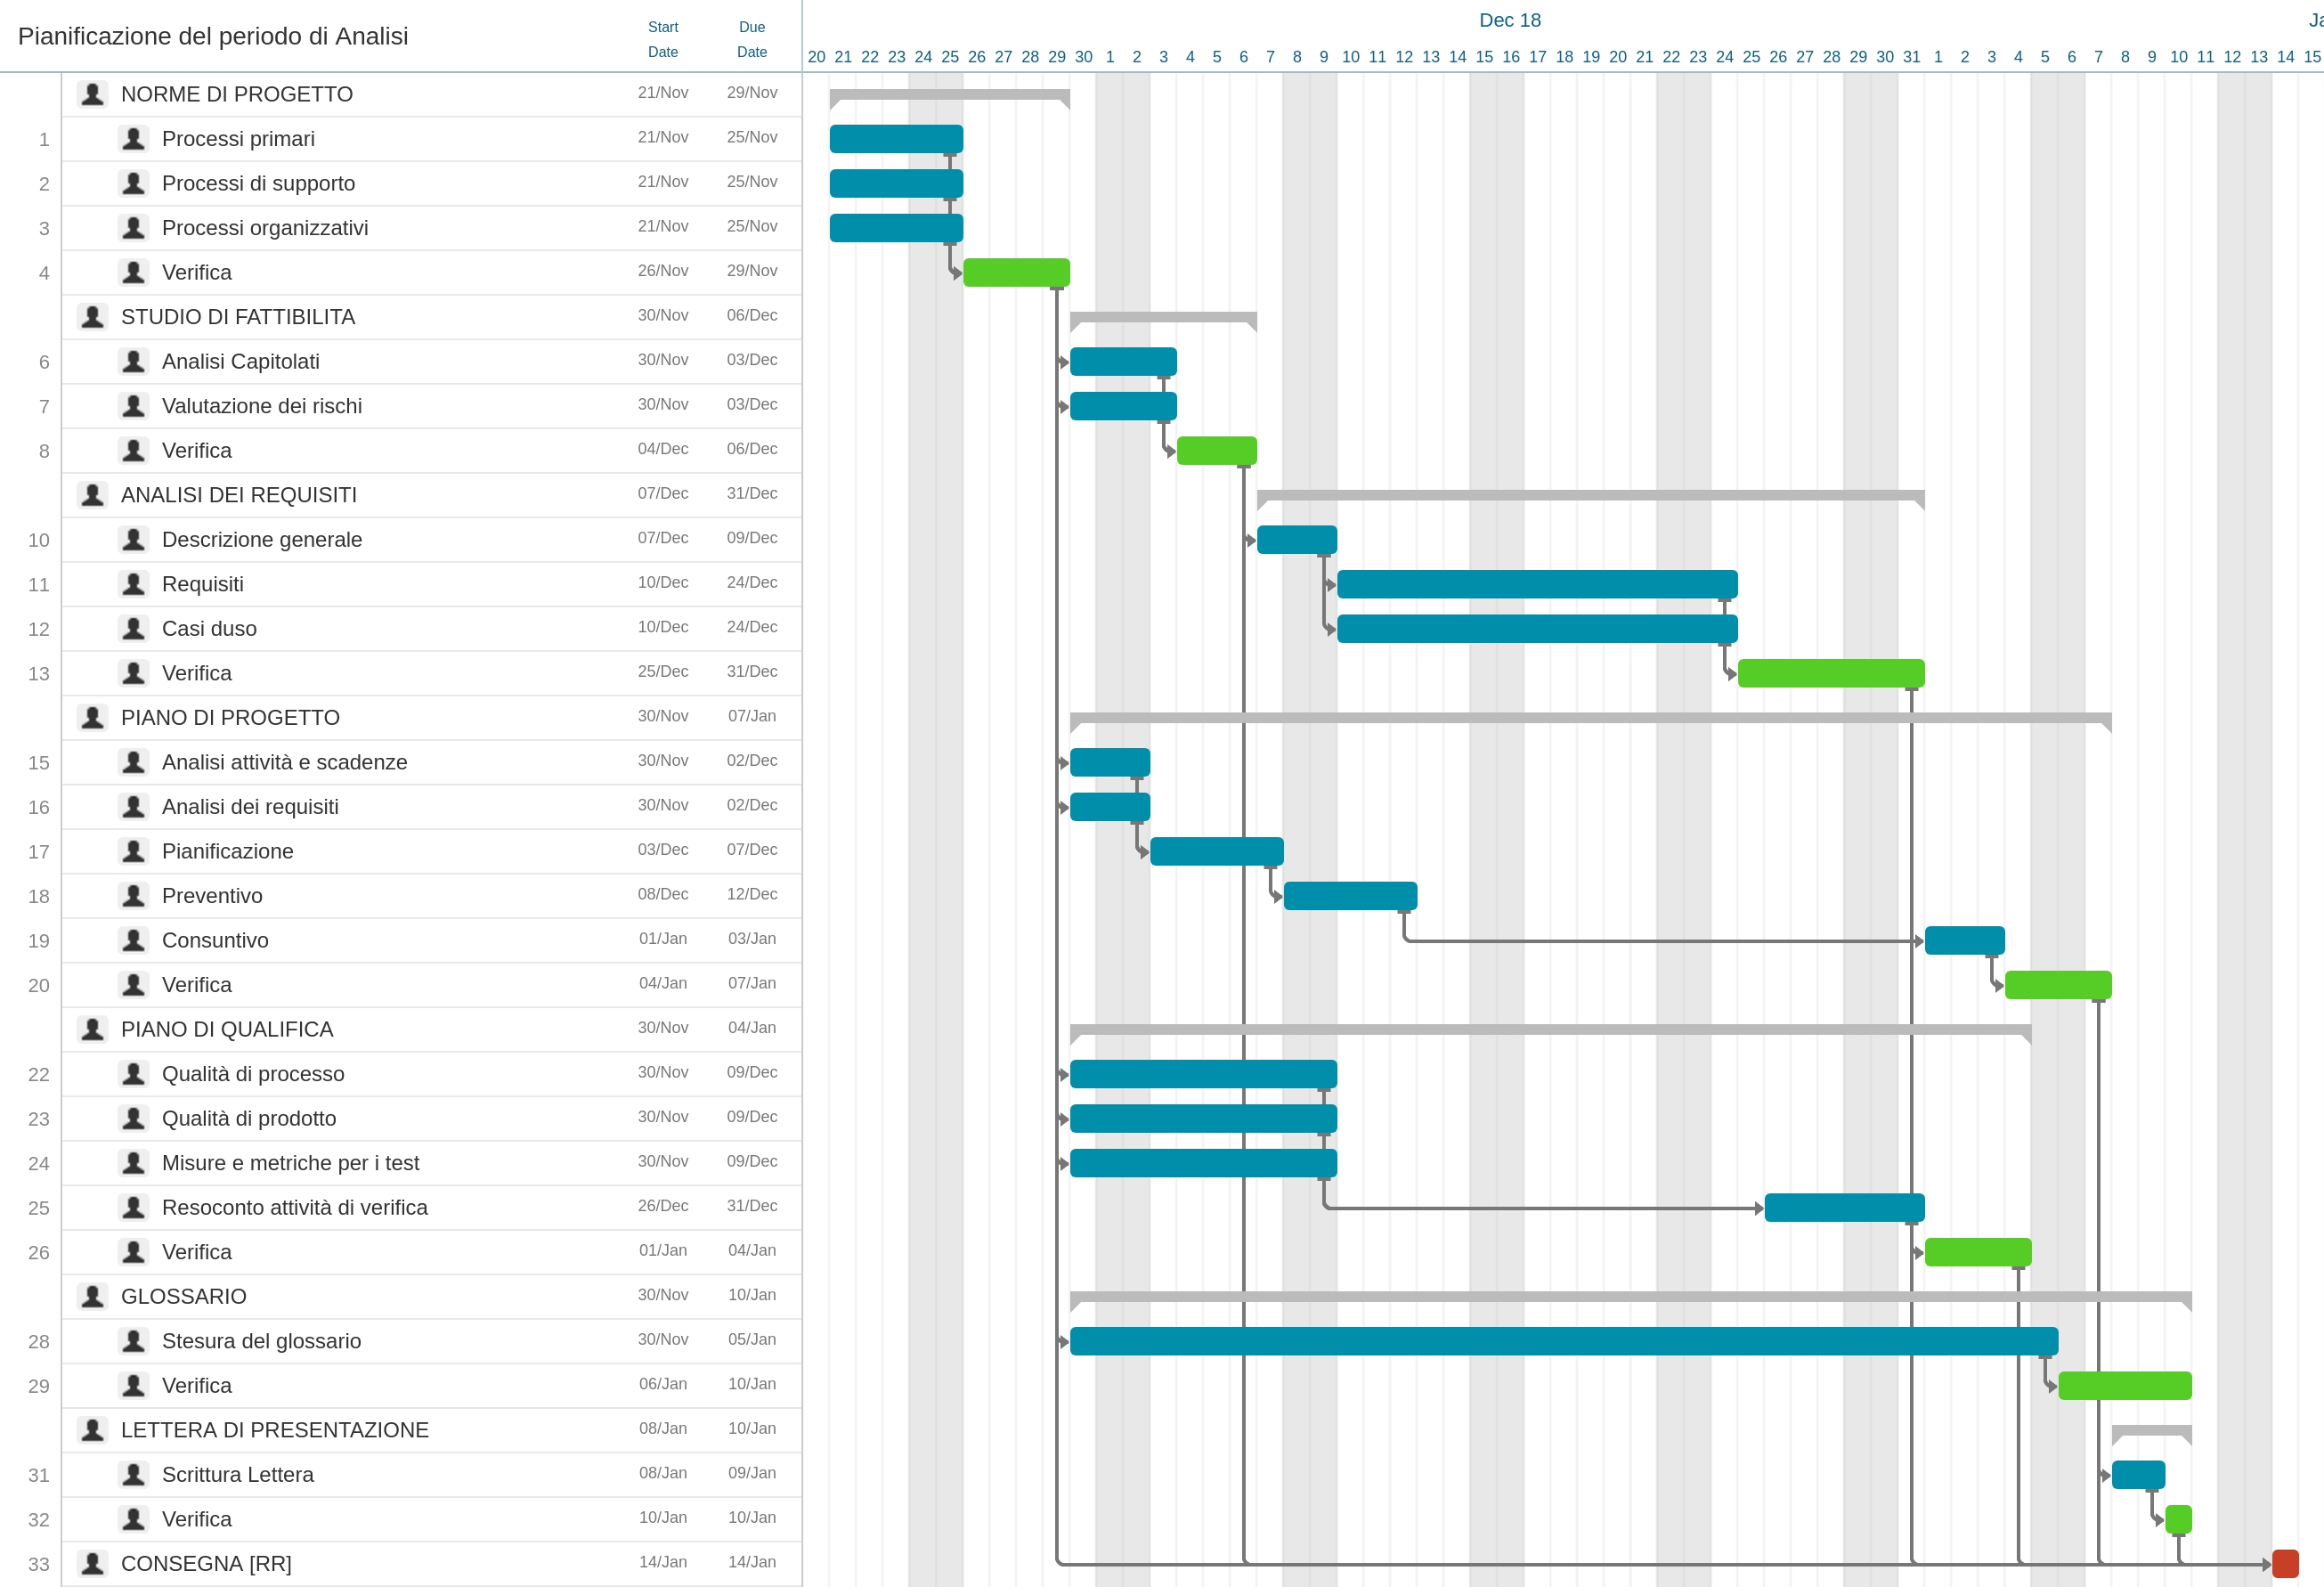
\includegraphics[width=15cm,keepaspectratio]{../includes/pics/grafici/Gantt_analisi.jpeg}
	\caption{\label{fig:mission}\markg{Diagramma di Gantt} del periodo di Analisi}
\end{figure}

\clearpage
\subsubsection{Consolidamento dei \markg{requisiti}}
La fase di consolidamento dei requisti ha inizio il 14-01-2019 con la consegna dei documenti per la prima scadenza e termina il 21-01-2019 con la presentazione della \emph{Revisione dei Requisiti}. Durante questo intervallo l'attività principale sarà il miglioramento dell'\emph{Analisi dei Requisiti} e dei documenti stilati in prospettiva dell'inizio del periodo di Progettazione della base applicativa richiesta.\\
\begin{figure}[htbp]
	\centering
	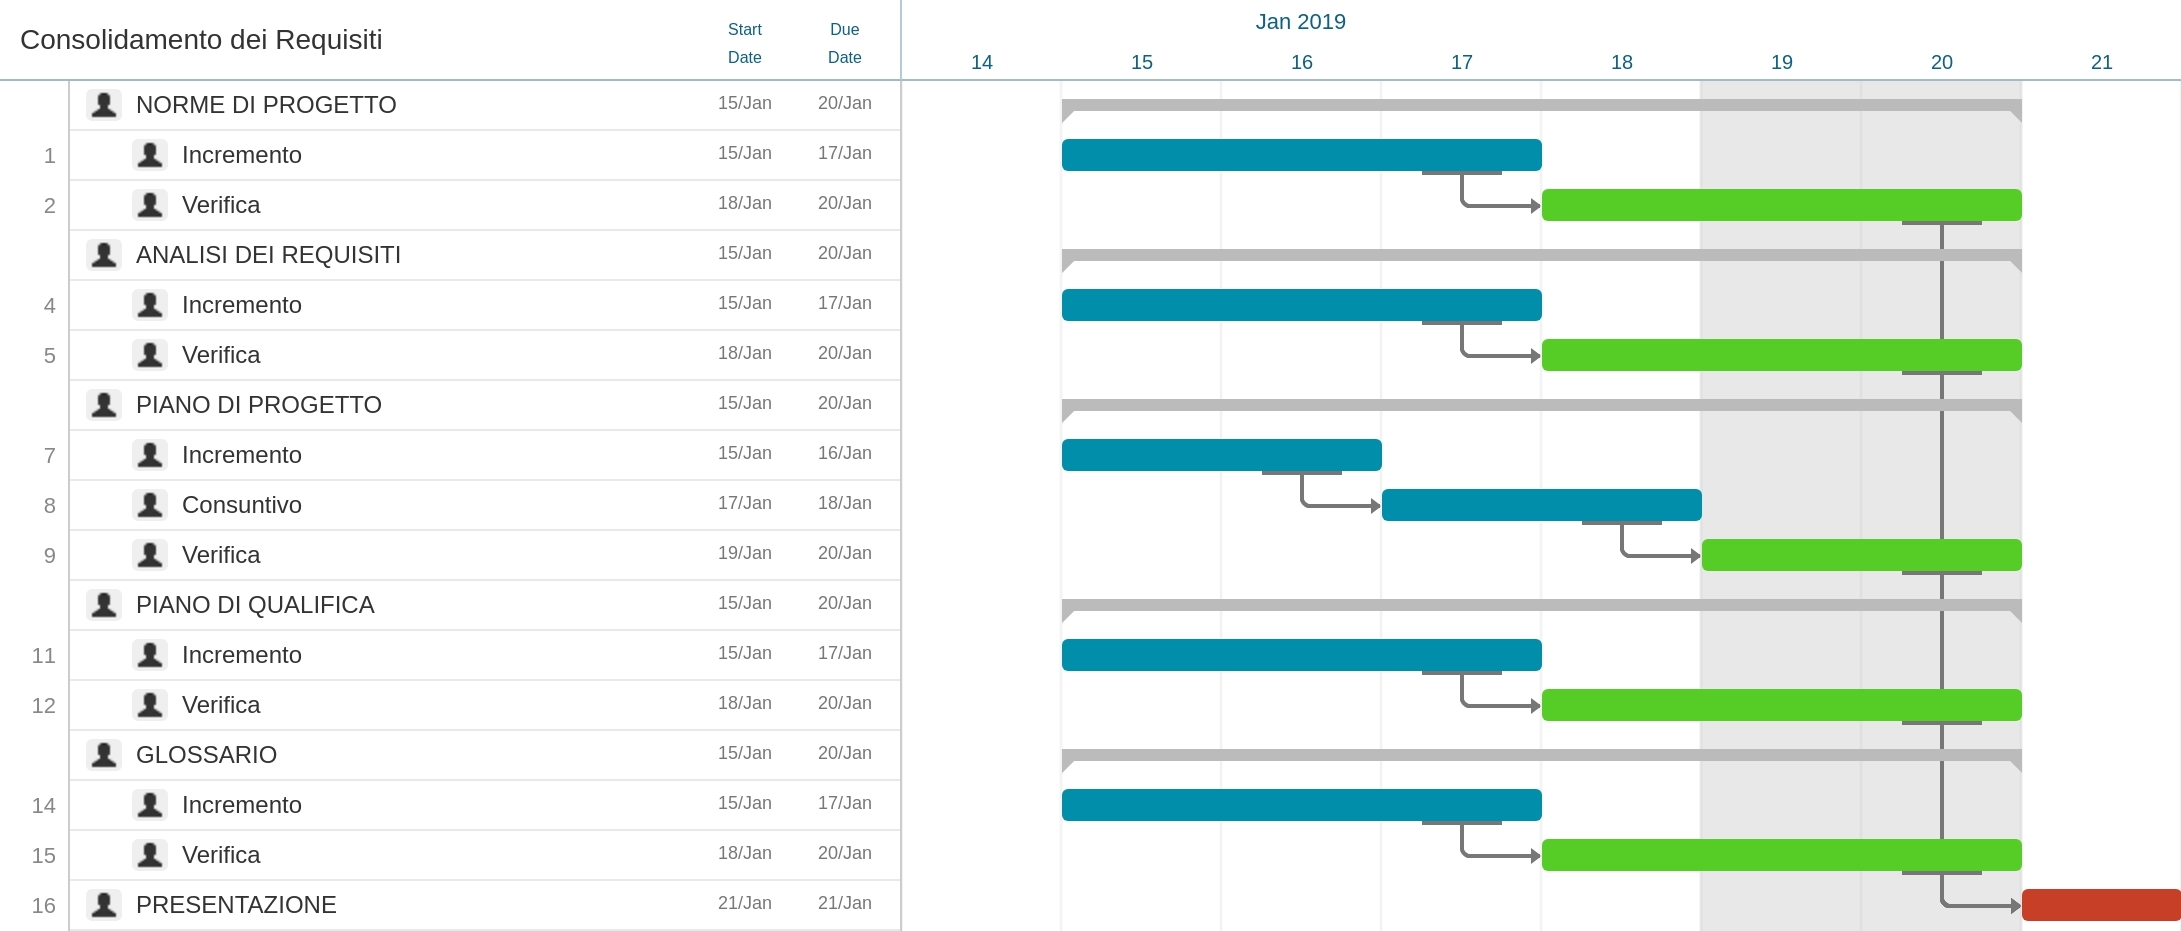
\includegraphics[width=15cm,keepaspectratio]{../includes/pics/grafici/Gantt_consolidamento_requisiti.jpeg}
	\caption{\label{fig:mission}\markg{Diagramma di Gantt} per il Consolidamento dei \markg{requisiti}}
\end{figure}

\clearpage
\subsection{Preventivo}
\subsubsection{Progettazione architetturale}
Durante l'intervallo di tempo che ha inizio il 22-01-2019, il giorno successivo la \emph{Revisione dei Requisiti}, e fine il 08-03-2019, termine consegna dei documenti per la \emph{Revisione di Progettazione}, verrà fatta la Progettazione della base tecnologica, le attività principali saranno:
	\begin{itemize}
		\item \textbf{Incremento e Verifica}: in questa attività, ad inizio periodo, vengono eseguite delle procedure di incremento e \markg{verifica} sui documenti \emph{Norme di Progetto, Analisi dei Requisisti, Piano di Progetto e Piano di Qualifica} seguendo le indicazioni risultanti dalla Revisione dei Requisiti. Dopo una elaborazione collettiva verrà stilato anche il documento \emph{Technology Baseline};
		\item \textbf{Lettera di presentazione}: in questa attività si prevede la stesura della Lettera di presentazione per la \emph{Revisione di Progettazione};
		\item \textbf{Technology Baseline}: in questa attività i Progettisti hanno il compito di scegliere le tecnologie, i \markg{framework} e le librerie di sviluppo per la realizzazione del prodotto e trascriverle nel documento \emph{Technology Baseline}. Tale attività è considerata determinante e critica per il conseguimento del progetto. Durante l'intervallo di tempo della \emph{Progettazione base tecnologica} verrà fatta una discussione per la \emph{\markg{verifica}} di tale documento;		
		\item \textbf{Glossario}: in questa attività vengono aggiunti nuovi termini e migliorato il \emph{Glossario}.
	\end{itemize}
\begin{figure}[htbp]
	\centering
	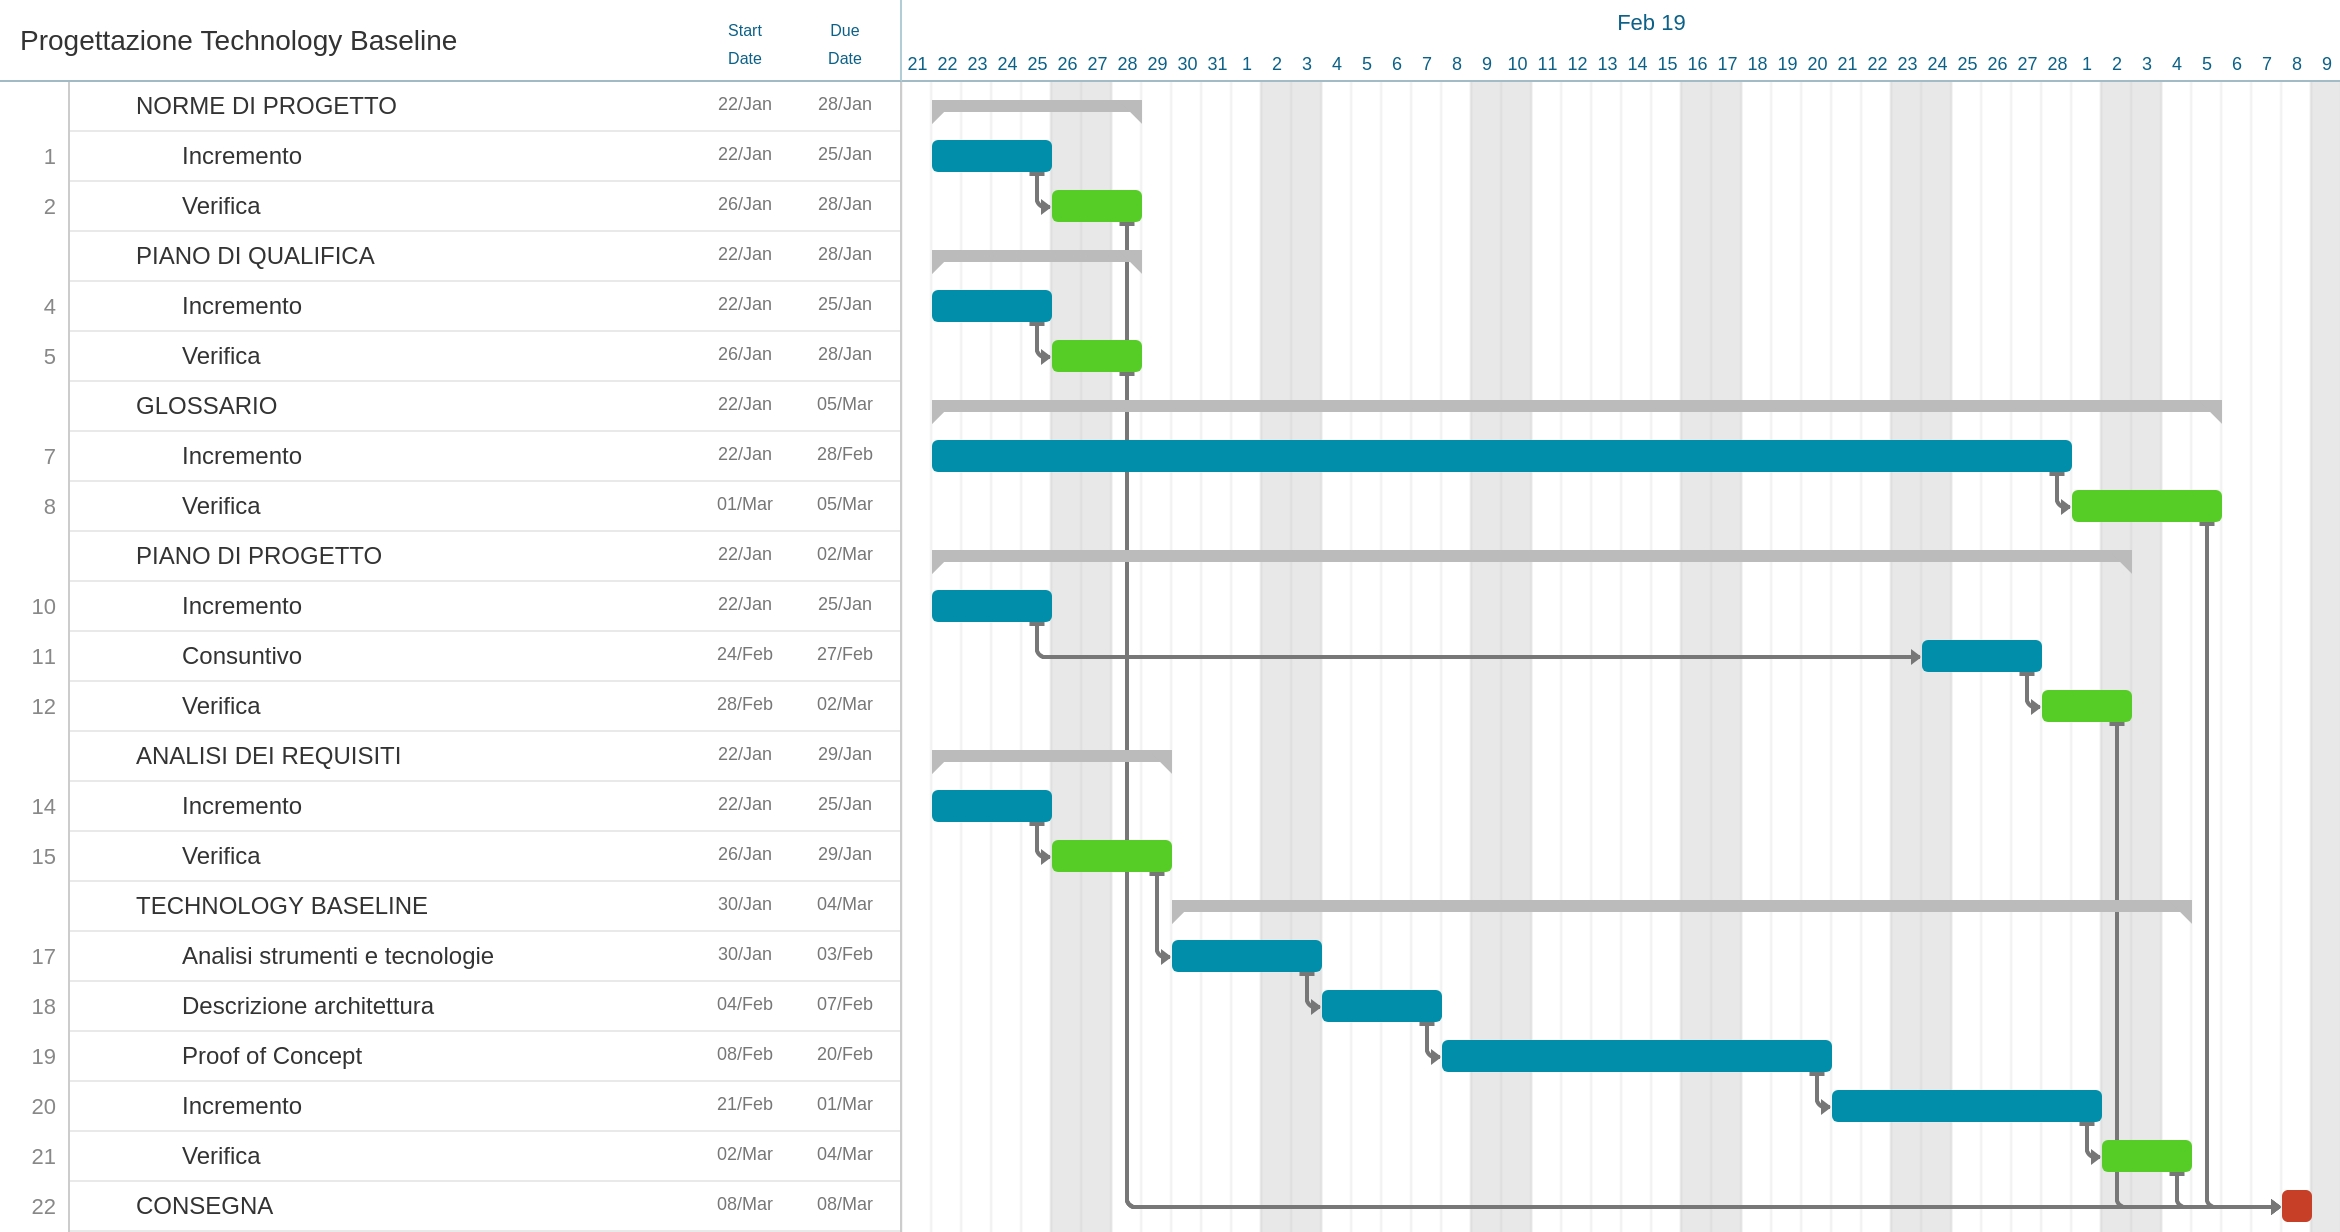
\includegraphics[width=15cm,keepaspectratio]{../includes/pics/grafici/Gantt_progettazione_technology_baseline.jpeg}
	\caption{\label{fig:mission}\markg{Diagramma di Gantt} Progettazione architetturale}
\end{figure}

\clearpage
\subsubsection{Progettazione di dettaglio e codifica}
Durante l'intervallo di tempo che ha inizio il 15-03-2019, il giorno stesso della \emph{Revisione di Progettazione}, e fine il 12-04-2019, termine consegna dei documenti per la \emph{Revisione di Qualifica}, verrà fatta la Progettazione di dettaglio e codifica, le cui attività principali saranno:
	\begin{itemize}
		\item \textbf{Incremento e Verifica}: in questa attività, ad inizio periodo, vengono eseguite delle procedure di incremento e \markg{verifica} sui documenti \emph{Norme di Progetto, Piano di Progetto, Piano di Qualifica e Technology Baseline} seguendo le indicazioni risultanti dalla Revisione dei Progettazione;
		\item \textbf{Lettera di presentazione}: in questa attività si prevede la stesura della Lettera di presentazione per la \emph{Revisione di Qualifica};
		\item \textbf{Product Baseline}: in questa attività si prevede la costruzione della \markg{baseline} architetturale del prodotto tramite diagrammi delle classi e di sequenza, va inoltre dimostrata la coerenza con quanto mostrato durante la \emph{Technology Baseline};
		\item \textbf{Codifica}: in questa attività è prevista la stesura del codice e la sua \emph{\markg{verifica}};
		\item \textbf{Manuale Utente}: in questa attività si prevede la realizzazione di un \emph{Manuale Utente} contenente indicazioni e direttive sull'utilizzo dell'applicazione prodotta;
		\item \textbf{Glossario}: in questa attività vengono aggiunti nuovi termini e migliorato il \emph{Glossario}.
	\end{itemize}
\begin{figure}[htbp]
	\centering
	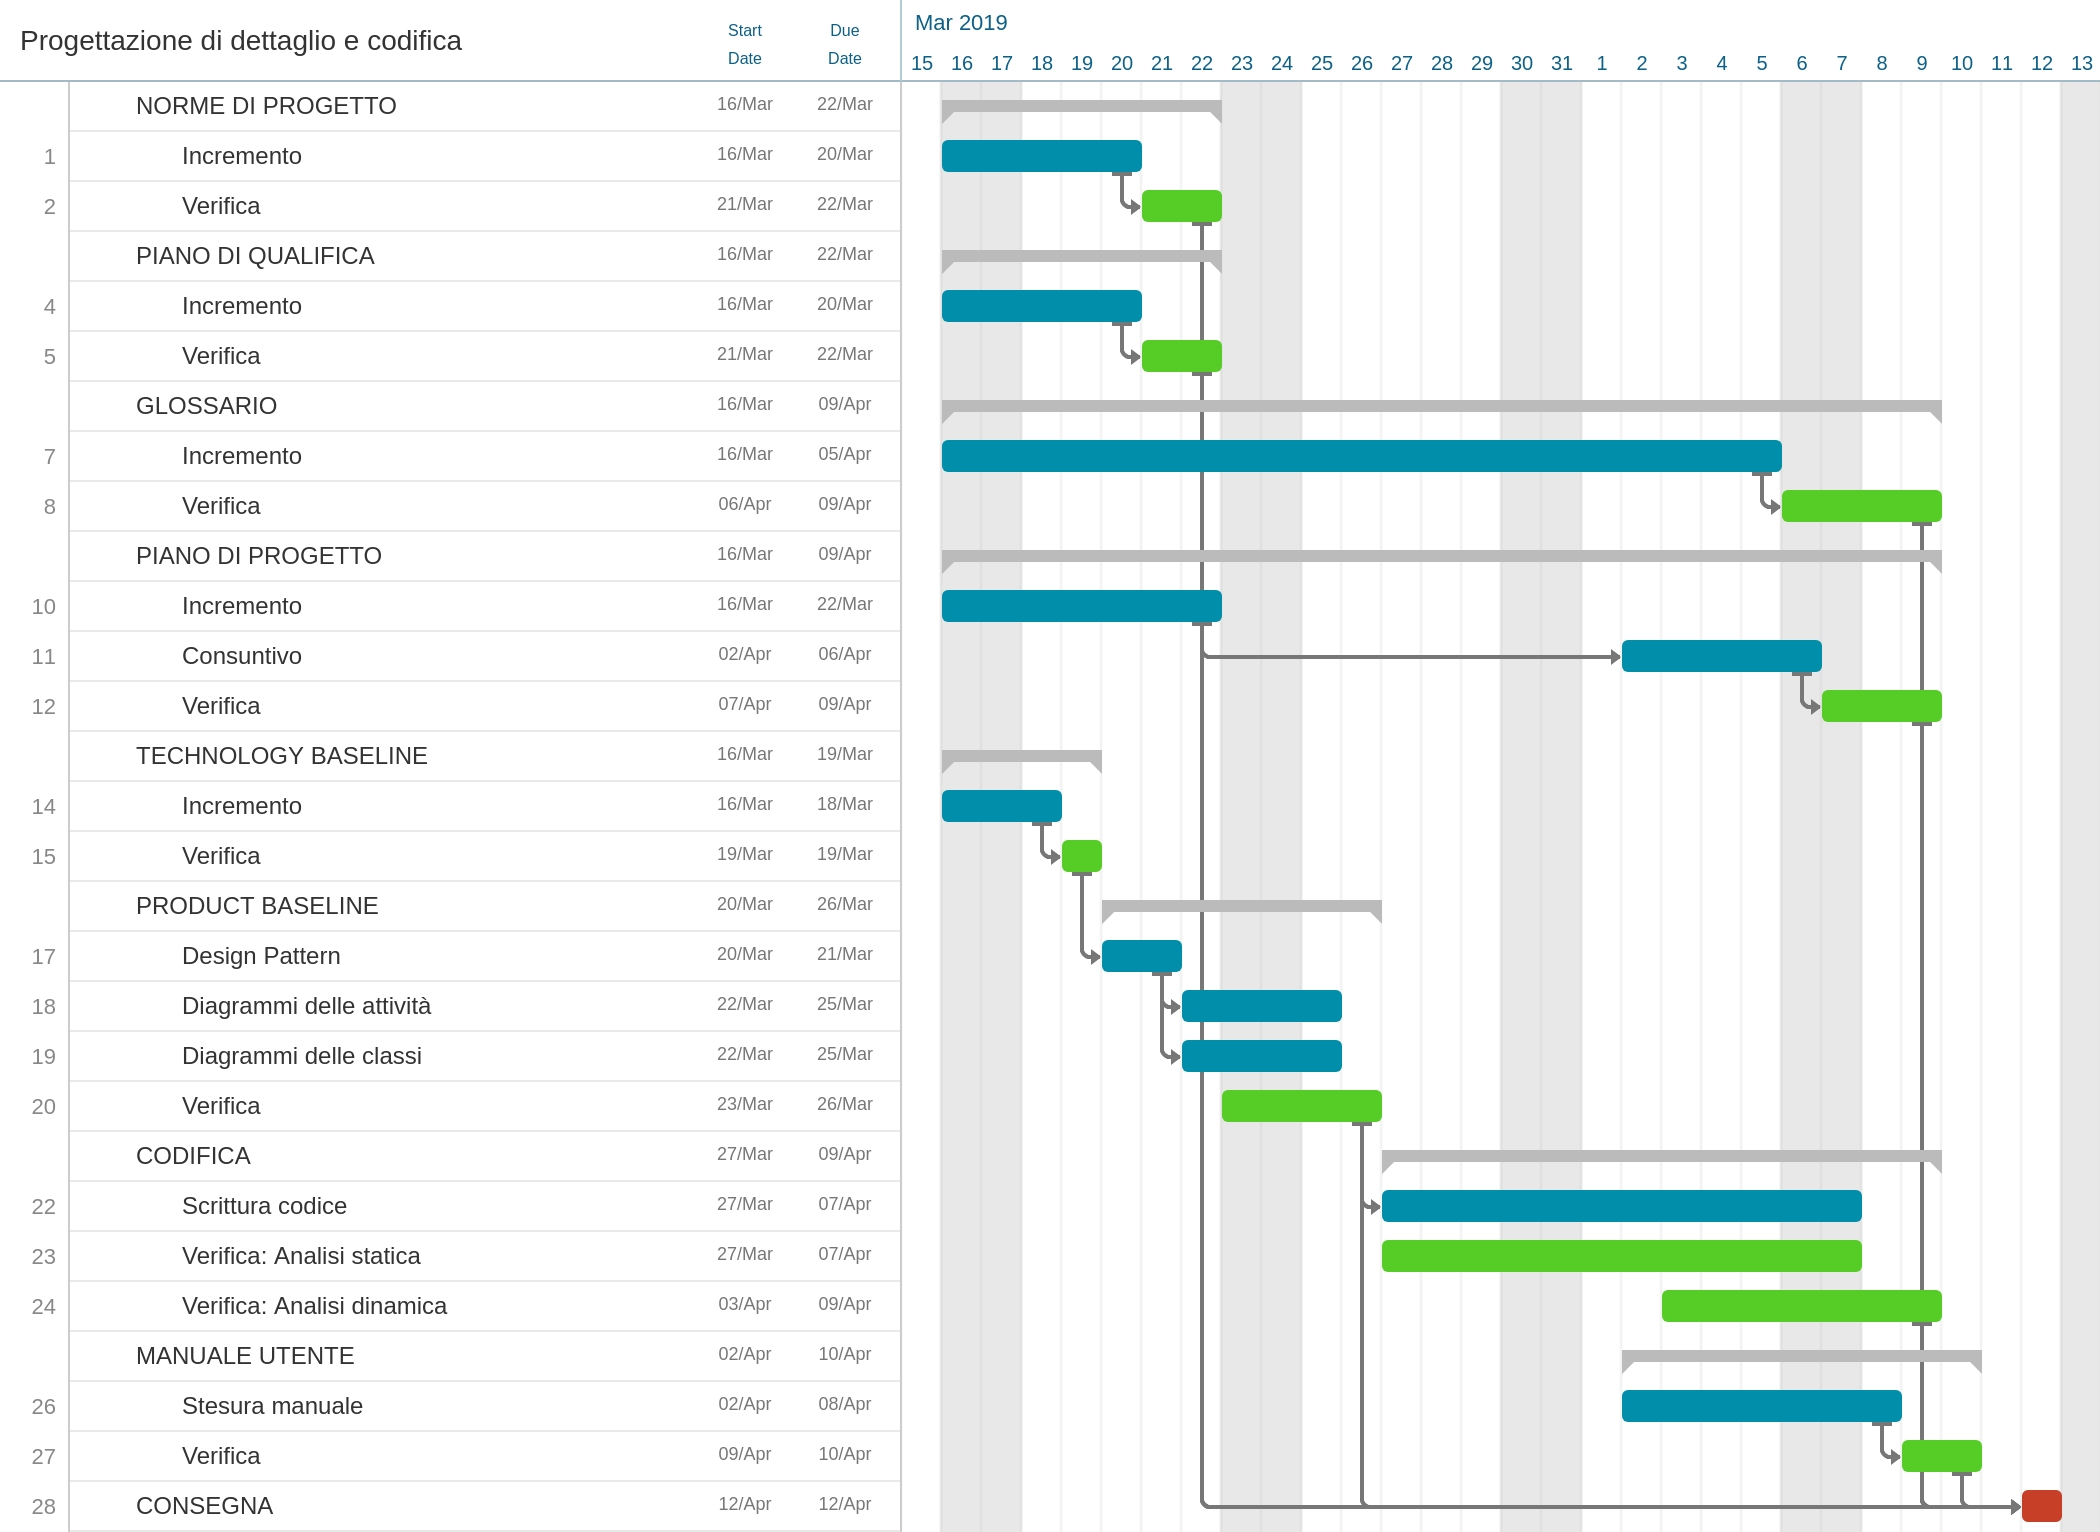
\includegraphics[width=15cm,keepaspectratio]{../includes/pics/grafici/Gantt_progettazione_dettaglio_codifica.jpeg}
	\caption{\label{fig:mission}\markg{Diagramma di Gantt} Progettazione di dettaglio e codifica}
\end{figure}

\clearpage
\subsubsection{Validazione e collaudo}
Durante l'intervallo di tempo che ha inizio il 19-04-2019, il giorno stesso della \emph{Revisione di Qualifica}, e fine il 10-05-2019, termine consegna dei documenti per la \emph{Revisione di Accettazione}, verranno svolti la \markg{validazione} ed il collaudo, le attività principali saranno:
\begin{itemize}
	\item \textbf{Incremento e Verifica}: in questa attività, ad inizio periodo, vengono eseguite delle procedure di incremento e \markg{verifica} sui documenti \emph{Norme di Progetto, Piano di Progetto, Piano di Qualifica e Product Baseline} seguendo le indicazioni risultanti dalla Revisione di Qualifica;
	\item \textbf{Validazione e Collaudo}: in questa attività è prevista l'esecuzione di test e miglioramenti dell'applicativo prodotto per garantire il soddisfacimento dei vincoli qualitativi;
	\item \textbf{Manuale Utente}: in questa attività si prevede la realizzazione di un \emph{Manuale Utente} contenente indicazioni e direttive sull'utilizzo dell'applicazione prodotta;
	\item \textbf{Glossario}: in questa attività vengono aggiunti nuovi termini e migliorato il \emph{Glossario}.
\end{itemize}
\begin{figure}[htbp]
	\centering
	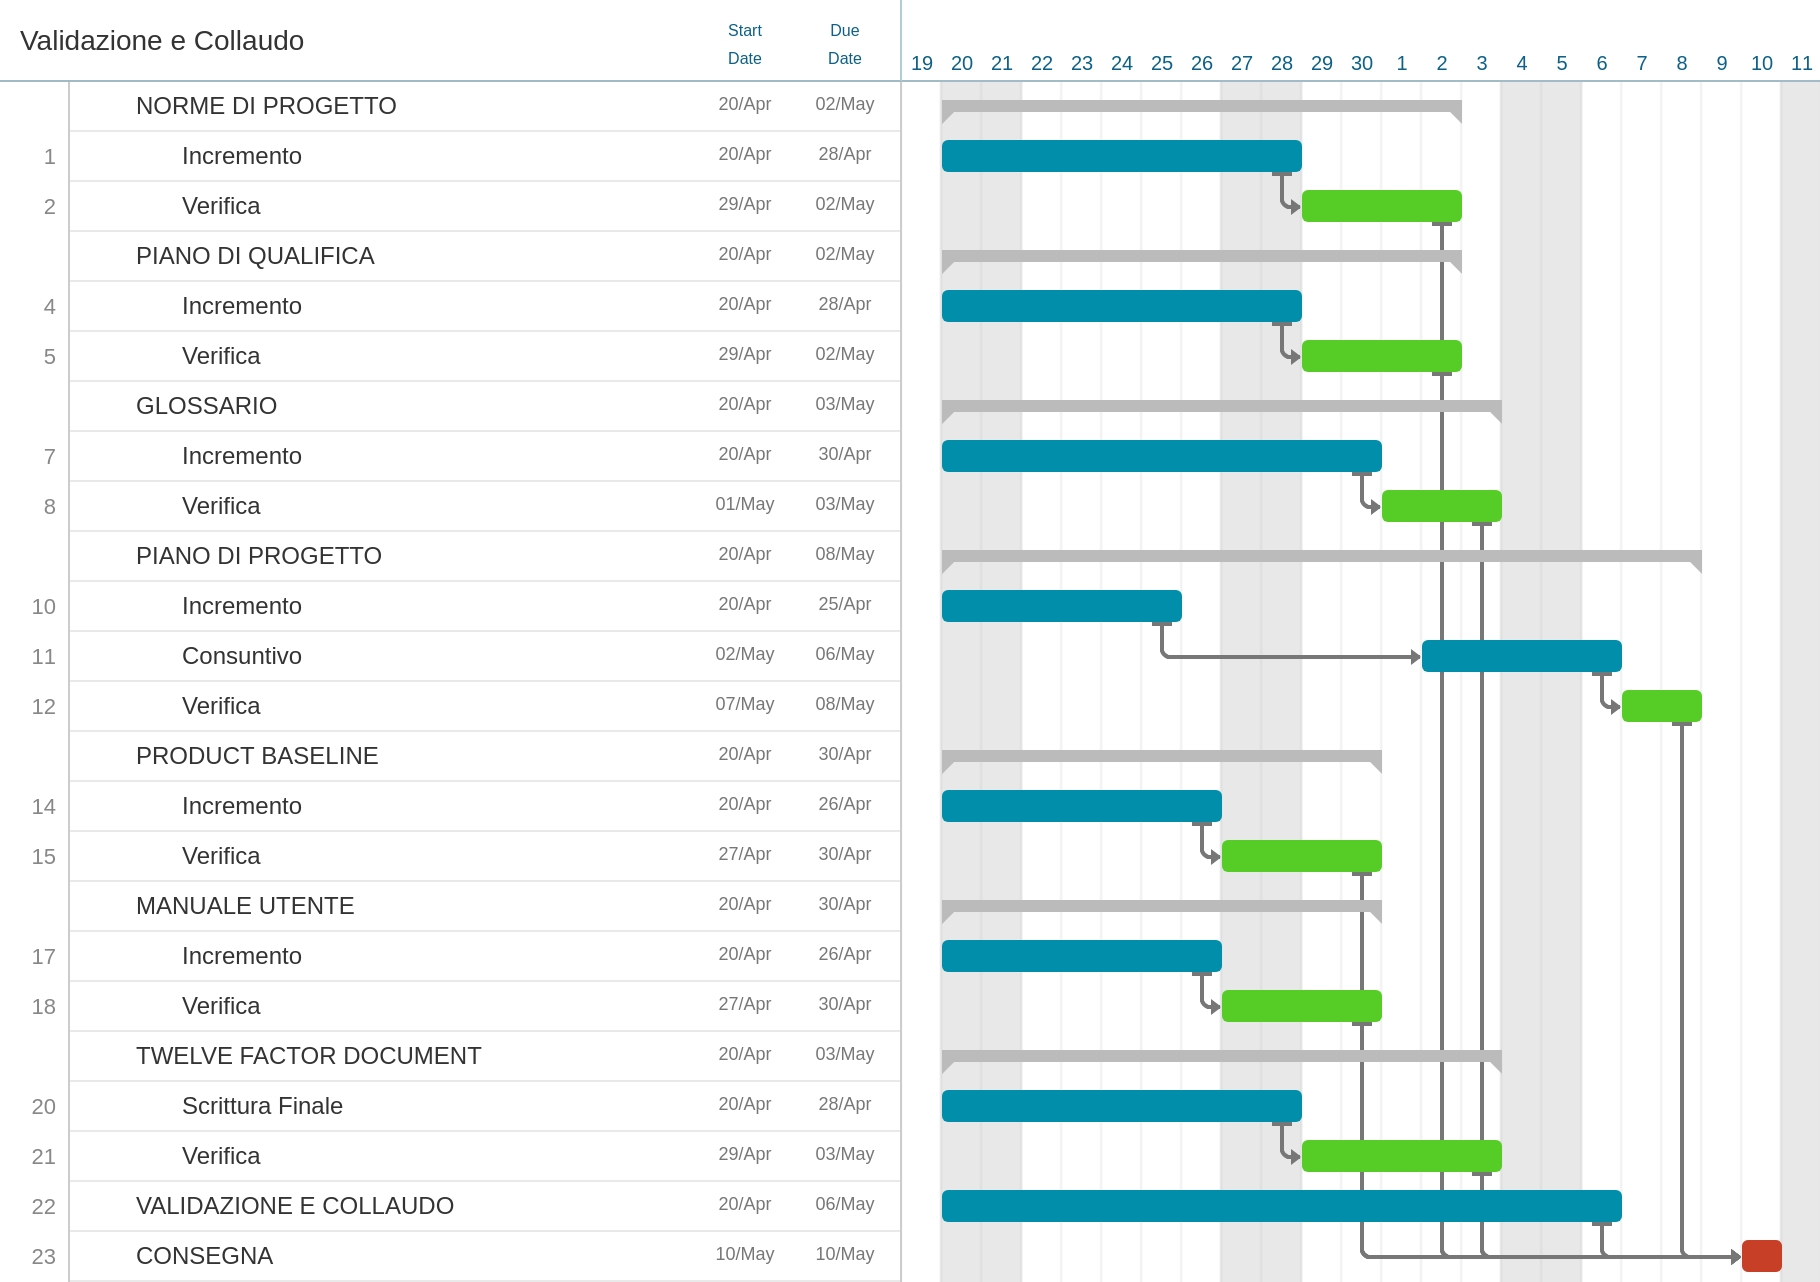
\includegraphics[width=15cm,keepaspectratio]{../includes/pics/grafici/Gantt_validazione_collaudo.jpeg}
	\caption{\label{fig:mission}\markg{Diagramma di Gantt} Validazione e collaudo}
\end{figure}
